\documentclass{article}
\usepackage{listings}
\usepackage{listings}
\usepackage{color}
\usepackage{graphicx}
\graphicspath{ {./} }
\usepackage[top=1in, bottom=1.25in, left=1.25in, right=1.25in]{geometry}
\definecolor{mygreen}{rgb}{0,0.6,0}
\definecolor{mygray}{rgb}{0.5,0.5,0.5}
\definecolor{mymauve}{rgb}{0.58,0,0.82}
\lstset{ %
	backgroundcolor=\color{white},   % choose the background color; you must add \usepackage{color} or \usepackage{xcolor}; should come as last argument
	basicstyle=\footnotesize,        % the size of the fonts that are used for the code
	breakatwhitespace=false,         % sets if automatic breaks should only happen at whitespace
	breaklines=true,                 % sets automatic line breaking
	captionpos=b,                    % sets the caption-position to bottom
	commentstyle=\color{mygreen},    % comment style
	deletekeywords={...},            % if you want to delete keywords from the given language
	escapeinside={\%*}{*)},          % if you want to add LaTeX within your code
	extendedchars=true,              % lets you use non-ASCII characters; for 8-bits encodings only, does not work with UTF-8
	frame=single,	                   % adds a frame around the code
	keepspaces=true,                 % keeps spaces in text, useful for keeping indentation of code (possibly needs columns=flexible)
	keywordstyle=\color{blue},       % keyword style
	language=Octave,                 % the language of the code
	morekeywords={*,...},            % if you want to add more keywords to the set
	numbers=left,                    % where to put the line-numbers; possible values are (none, left, right)
	numbersep=5pt,                   % how far the line-numbers are from the code
	numberstyle=\tiny\color{mygray}, % the style that is used for the line-numbers
	rulecolor=\color{black},         % if not set, the frame-color may be changed on line-breaks within not-black text (e.g. comments (green here))
	showspaces=false,                % show spaces everywhere adding particular underscores; it overrides 'showstringspaces'
	showstringspaces=false,          % underline spaces within strings only
	showtabs=false,                  % show tabs within strings adding particular underscores
	stepnumber=2,                    % the step between two line-numbers. If it's 1, each line will be numbered
	stringstyle=\color{mymauve},     % string literal style
	tabsize=2,	                   % sets default tabsize to 2 spaces
	title=\lstname                   % show the filename of files included with \lstinputlisting; also try caption instead of title
}
\author{Polykarpos Thomadakis}
\title{Assignment 3 \\
	\large CS834 Introduction to Information Retrieval\\Fall 2017}

\begin{document}
	\maketitle
	\section*{Question 6.1}
	Using theWikipedia collection provided at the book website, create a sample
	of stem clusters by the following process:
	\begin{enumerate}
	\item Index the collection without stemming.
	\item  Identify the first 1,000 words (in alphabetical order) in the index.
	\item Create stem classes by stemming these 1,000 words and recording which words become the same stem.
	\item Compute association measures (Dice’s coefficient) between all pairs of stems in each stem class. Compute co-occurrence at the document level.
	\item Create stem clusters by thresholding the association measure. All terms that are still connected to each other form the clusters.
	\end{enumerate}
	Compare the stem clusters to the stem classes in terms of size and the quality (in your opinion) of the groupings.
	\subsection*{Answer}
	For this assignment, I used the code I used in assignment 2 to produce the inverted index. Then, I sort the index alphabetically and pick the first 1000 words and create stems from each one of them using the krovetz stemmer. Once I have created the stems, I create bigrams from them in order to find co-occurences in the given collection and apply Dice's coefficient to create the stemming clusters. I set the threshold to 0.01 and then extracted the connected subgraphs produced by the code. The code used can be seen in listing \ref{lst:dice_clust}.
	\lstinputlisting[language=Python,caption={Script to extract the stem clusters using Dice's coefficient},label={lst:dice_clust}]{dice_stem_clusters.py}
	The clusters created by the algorithm are presented in table \ref{tb:dice_clusters}.
	\begin{table}[h]
	\centering
	\caption{Clusters created using the Dice's coefficient on the small wikipedia collection}
	\label{tb:dice_clusters}
	\begin{tabular}{|l|l|}
	\hline
	academician  & Academician,Academicians    \\ \hline
	abbott       & Abbotts,Abbott              \\ \hline
	abstraction  & Abstraction,Abstractions    \\ \hline
	abugida      & Abugidas,Abugida            \\ \hline
	acquisition  & Acquisitions,Acquisition    \\ \hline
	ace          & Aces,Acer                   \\ \hline
	actor        & Actors,Actor                \\ \hline
	acronym      & Acronym,Acronyms            \\ \hline
	access       & Access,Accessed             \\ \hline
	account      & Accounting,Account,Accounts \\ \hline
	abbey        & Abbeys,Abbey                \\ \hline
	abbreviation & Abbreviation,Abbreviations  \\ \hline
	accident     & Accident,Accidents          \\ \hline
	abt          & Abts,Abt                    \\ \hline
	absurd       & Absurdity,Absurd            \\ \hline
	acre         & Acres,Acre                  \\ \hline
	atpase       & ATPase,ATPases              \\ \hline
	activity     & Activities,Activity         \\ \hline
	achievement  & Achievements,Achievement    \\ \hline
	adaboost     & AdaBoost,Adaboost           \\ \hline
	\end{tabular}
	\end{table}
	\section*{Question 6.2}
	Create a simple spelling corrector based on the noisy channel model. Use a
	single-word language model, and an error model where all errors with the same
	edit distance have the same probability. Only consider edit distances of 1 or 2.
	Implement your own edit distance calculator (example code can easily be found
	on the Web).
	\subsection*{Answer}
	For the edit distance calculator I used the python code found in \textit{http://norvig.com/spell-correct.html}, specifically edits1 and edits2, that which given a misspelled word apply 1 and 2 letter transformations to the misspelled word with the purpose of generating a valid one. Once I collect the set of words generated this way, I keep only those that are valid words by checking if they exist in a big collection of words in file \textit{big.txt} found in the repository (adopted from the same site noted above). Once the valid words have been collected, I compute the probability the frequency that each of those words appears, and finally correct the misspelled word with the most frequent word of the set of valid words collected. The code for this assignment appears in listing \ref{lst:spell_correction}.
	\lstinputlisting[language=Python,caption={Script to correct a misspelled word based on the noisy channel model},label={lst:spell_correction}]{spell_correction.py}
	Figure \ref{fig:spell_correction} demonstrates the spell correction program listed above.
	\begin{figure}[h]
		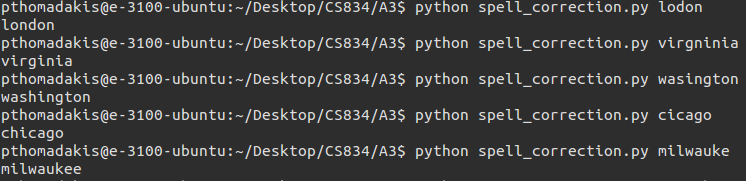
\includegraphics[width=\linewidth]{spell_correction.png}
		\caption{Sample output of the spell correction script}
		\label{fig:spell_correction}
	\end{figure}
	\section*{Question 6.5}
	Describe the snippet generation algorithm in Galago. Would this algorithm
	work well for pages with little text content? Describe in detail how you would
	modify the algorithm to improve it.
	\subsection*{Answer}
	The code for the Galago search engine can be found in \textit{https://storage.googleapis.com/google-code-archive-downloads/v2/code.google.com/galagosearch/galagosearch-1.04-src.tar.gz}. The code for the snippet generation resides in the file: \\ \textit{galagosearch-1.04/galagosearch-core/src/main/java/org/galagosearch/core/store/SnippetGenerator.java}.\\
	The algorithm can be described as the following 6 steps:
	\begin{enumerate}
		\item Tokenize the document into terms and maintain them and their positions.
		\item Find all the terms in the document that match the ones of the query.
		\item When a term is matched, retrieve a small region of the document that contains the term.
		\item Check for overlapping regions and merge them if any.
		\item Keep adding document regions to the snippet, until the maximum size is reached.
		\item Combine all regions to a single html string.
	\end{enumerate}
	Galago includes snippets only when the exact term is found in the document. Thus, when a small document is indexed there is a lower probability that a term will appear and as a result a lower probability that a snippet will be generated. Also, Galago does not seem to use stemming, meaning that it is even less probable for a snippet to be generated. In my oppinion, stemming would increase the quality of snippet generation as it does for searching. If this also fails, it would be a good attempt to just display the first few sentences of the document. Since it has already been marked as relevant, it makes sense that at the introduction of the document there will be some reference relevant to the query term.
	\section*{Question MLN1}
	Using the small wikipedia example, choose 10 words and create stem classes as per the algorithm on pp. 191-192.
	\subsection*{Answer}
	This assignment can be answered directly using the code from question 6.1. To add more value to the code used there I added the stem clusters produced when other association metrics are used, namely Dice's coefficient, EMIM, MIM and Chi-square. \\The ten words I randomly chose are:\\ \textquotedblleft academician\textquotedblright ,\textquotedblleft university\textquotedblright, \textquotedblleft mind\textquotedblright, \textquotedblleft synonym\textquotedblright, \textquotedblleft monitor\textquotedblright, \textquotedblleft owe\textquotedblright,  \textquotedblleft top\textquotedblright ,\textquotedblleft charge\textquotedblright ,\textquotedblleft hit\textquotedblright ,\textquotedblleft diverge\textquotedblright.\\
	Figure \ref{fig:10_word_stem_classes} shows the classes created from each metric using threshold 0.01. The code used for this assignment is shown in listing \ref{lst:10_word_stem_classes}
	\lstinputlisting[language=Python,caption={Script to generate stem classes for the 10 chosen words},label={lst:10_word_stem_classes}]{10_word_stem_classes.py}
	\begin{figure}[h!]
		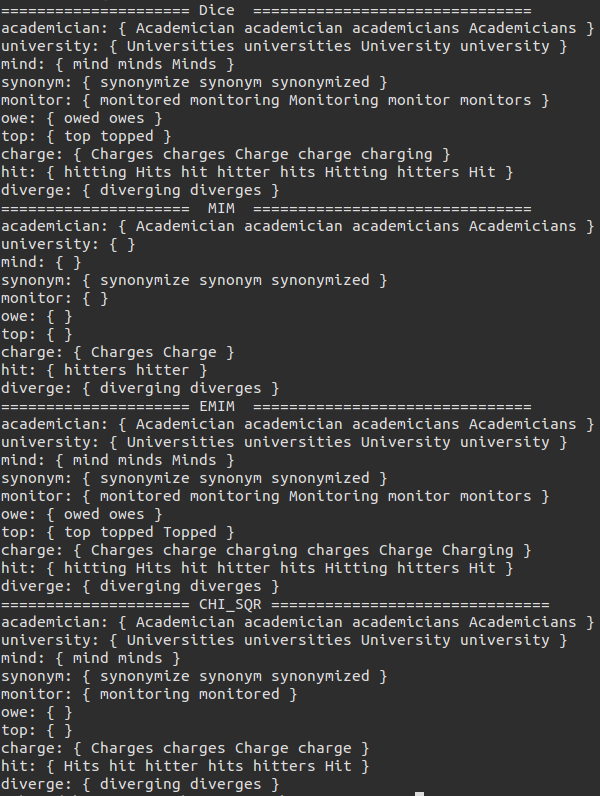
\includegraphics[width=\linewidth]{10_stem_classes.png}
		\caption{Stem classes produced for different association metrics}
		\label{fig:10_word_stem_classes}
	\end{figure}
	\section*{Question MLN2}
	 Using the small wikipedia example, choose 10 words and compute MIM, EMIM, chi square, dice association measures for full document and 5 word windows (cf. pp. 203-205)
	\subsection*{Answer}
	The script that was written for this assignment can be found in listing \ref{lst:10_word_associates}. It uses the inverted index of the previous assignments (or regenerates it if it does not exist) to calculate the association measures using the metrics: MIM, EMIM, Chi-squared and Dice's coefficient. The ten words I randomly chose are:
	\textquotedblleft instrument\textquotedblright,\textquotedblleft university\textquotedblright,\textquotedblleft book\textquotedblright,\textquotedblleft America\textquotedblright,\textquotedblleft fish\textquotedblright,\textquotedblleft dinosaur\textquotedblright,\textquotedblleft car\textquotedblright,\textquotedblleft food\textquotedblright,\textquotedblleft hit\textquotedblright,\textquotedblleft soccer\textquotedblright.
	\lstinputlisting[language=Python,caption={Script to generate top 10 associated words for the 10 chosen words},label={lst:10_word_associates}]{10_word_associates.py}
	The resulting associated words are shown in tables \ref{tb:instrument}-\ref{tb:soccer}.	We can see that the associated words can differ significantly depending on the metric that is used to measure association. The most significant difference in the table is noticed on the MIM metric, where almost none of the words is common with the other ones. That is probably caused by the fact that this metric favors low-frequency terms, since $n_a*n_b$ will increase very fast for frequent words a,b but their co-occurrence remains the same. As a result, the total value will be very low compared to low-frequency.
	\begin{table}[h]
	\centering
	\caption{Associated words for word \textquotedblleft instrument\textquotedblright}
	\label{tb:instrument}
	\resizebox{0.8\linewidth}{!}{
	\begin{tabular}{|l|l|l|l|}
	\hline
	\multicolumn{4}{|c|}{instrument}                                                                             \\ \hline
	\multicolumn{1}{|c|}{Dice} & \multicolumn{1}{c|}{MIM} & \multicolumn{1}{c|}{EMIM} & \multicolumn{1}{c|}{Chi} \\ \hline
	instruments                & Mortem                   & instruments               & instruments              \\ \hline
	signature                  & Serwaczynski             & musical                   & timbres                  \\ \hline
	Perspectives               & conductive               & music                     & Buggles                  \\ \hline
	Furrykef                   & Jbonneau                 & such                      & ney                      \\ \hline
	scores                     & Desinicization           & some                      & Postmodernism            \\ \hline
	Instrument                 & Arhielanto               & used                      & disclosed                \\ \hline
	sensitive                  & Dentine                  & up                        & Ulmanor                  \\ \hline
	musical                    & Artisan                  & heavily                   & halts                    \\ \hline
	Face                       & Dannycali                & different                 & Crazed                   \\ \hline
	timbres                    & SatellitesHidden         & various                   & Maxillofacial            \\ \hline
	\end{tabular}
	}
	\end{table}
	\begin{table}[h]
	\centering
	\caption{Associated words for word \textquotedblleft university\textquotedblright}
	\label{tb:university}
	\resizebox{0.8\linewidth}{!}{
	\begin{tabular}{|l|l|l|l|}
	\hline
	\multicolumn{4}{|c|}{university}                                                                             \\ \hline
	\multicolumn{1}{|c|}{Dice} & \multicolumn{1}{c|}{MIM} & \multicolumn{1}{c|}{EMIM} & \multicolumn{1}{c|}{Chi} \\ \hline
	institution                & Tootie                   & University                & institution              \\ \hline
	universities               & Pamplemousse             & education                 & universities             \\ \hline
	campus                     & Mortem                   & college                   & education                \\ \hline
	academic                   & Velocisaurus             & institution               & campus                   \\ \hline
	education                  & Cheiro                   & students                  & academic                 \\ \hline
	college                    & Babineau                 & campus                    & college                  \\ \hline
	student                    & Wingwangwo               & academic                  & postgraduate             \\ \hline
	colleges                   & Malfatti                 & universities              & Faculties                \\ \hline
	Engineering                & majr                     & College                   & University               \\ \hline
	students                   & Thegreyanomaly           & student                   & colleges                 \\ \hline
	\end{tabular}
	}
	\end{table}
	\begin{table}[]
	\centering
	\caption{Associated words for word \textquotedblleft book\textquotedblright}
	\label{tb:book}
	\resizebox{0.8\linewidth}{!}{
	\begin{tabular}{|l|l|l|l|}
	\hline
	\multicolumn{4}{|c|}{book}                                                                                   \\ \hline
	\multicolumn{1}{|c|}{Dice} & \multicolumn{1}{c|}{MIM} & \multicolumn{1}{c|}{EMIM} & \multicolumn{1}{c|}{Chi} \\ \hline
	published                  & Simka                    & published                 & published                \\ \hline
	books                      & Mortem                   & books                     & books                    \\ \hline
	story                      & SparrowsWing             & story                     & story                    \\ \hline
	written                    & fiction                  & his                       & novels                   \\ \hline
	novel                      & Pvasiliadis              & written                   & novel                    \\ \hline
	author                     & Mucks                    & he                        & comic                    \\ \hline
	wrote                      & Norilana                 & that                      & author                   \\ \hline
	Books                      & Grecque                  & novel                     & fiction                  \\ \hline
	series                     & author                   & they                      & Publication              \\ \hline
	Book                       & equilateral              & author                    & wrote                    \\ \hline
	\end{tabular}
	}
	\end{table}
	\begin{table}[]
	\centering
	\caption{Associated words for word \textquotedblleft America\textquotedblright}
	\label{tb:america}
	\resizebox{0.8\linewidth}{!}{
	\begin{tabular}{|l|l|l|l|}
	\hline
	\multicolumn{4}{|c|}{America}                                                                                \\ \hline
	\multicolumn{1}{|c|}{Dice} & \multicolumn{1}{c|}{MIM} & \multicolumn{1}{c|}{EMIM} & \multicolumn{1}{c|}{Chi} \\ \hline
	North                      & Tootie                   & North                     & North                    \\ \hline
	American                   & Mortes                   & American                  & Europe                   \\ \hline
	Europe                     & Mortem                   & New                       & Asia                     \\ \hline
	New                        & seamier                  & show                      & American                 \\ \hline
	York                       & Sergeants                & States                    & Oceania                  \\ \hline
	through                    & Pinkerton                & hide                      & Mexico                   \\ \hline
	States                     & Mucko                    & var                       & Brazil                   \\ \hline
	most                       & Zizaniopsis              & tocShowText               & York                     \\ \hline
	South                      & Velocisaurus             & showTocToggle             & Africa                   \\ \hline
	began                      & Amirthanayagam           & tocHideText               & New                      \\ \hline
	\end{tabular}
	}
	\end{table}
	\begin{table}[]
	\centering
	\caption{Associated words for word \textquotedblleft fish\textquotedblright}
	\label{tb:fish}
	\resizebox{0.8\linewidth}{!}{
	\begin{tabular}{|l|l|l|l|}
	\hline
	\multicolumn{4}{|c|}{fish}                                                                                   \\ \hline
	\multicolumn{1}{|c|}{Dice} & \multicolumn{1}{c|}{MIM} & \multicolumn{1}{c|}{EMIM} & \multicolumn{1}{c|}{Chi} \\ \hline
	Actinopterygii             & hukim                    & species                   & Actinopterygii           \\ \hline
	Fish                       & Keulemans                & Actinopterygii            & FishBase                 \\ \hline
	Chordata                   & desiccant                & water                     & Ranier                   \\ \hline
	freshwater                 & Jabr                     & Chordata                  & Osteichthyes             \\ \hline
	species                    & Sennet                   & Fish                      & Fishes                   \\ \hline
	Phylum                     & Percopsiformes           & Phylum                    & Fish                     \\ \hline
	fins                       & bellow                   & classification            & Pauly                    \\ \hline
	Animalia                   & ars\={e}n                & Animalia                  & fins                     \\ \hline
	FishBase                   & Protista                 & Scientific                & fin                      \\ \hline
	Ranier                     & bobwhite                 & Family                    & Froese                   \\ \hline
	\end{tabular}
	}
	\end{table}
	\begin{table}[]
	\centering
	\caption{Associated words for word \textquotedblleft dinosaur\textquotedblright}
	\label{tb:dinosaur}
	\resizebox{0.8\linewidth}{!}{
	\begin{tabular}{|l|l|l|l|}
	\hline
	\multicolumn{4}{|c|}{dinosaur}                                                                               \\ \hline
	\multicolumn{1}{|c|}{Dice} & \multicolumn{1}{c|}{MIM} & \multicolumn{1}{c|}{EMIM} & \multicolumn{1}{c|}{Chi} \\ \hline
	Dinosaurs                  & Velocisaurus             & dinosaurs                 & Dinosaurs                \\ \hline
	dinosaurs                  & Cucumber                 & Dinosaurs                 & dinosaurs                \\ \hline
	theropod                   & Gurche                   & Firsfron                  & theropod                 \\ \hline
	Dinosauria                 & jil                      & theropod                  & Dinosauria               \\ \hline
	Cretaceous                 & candelariensis           & Dinosauria                & Saurischia               \\ \hline
	Sauropsida                 & sauropodomorph           & Spencer                   & Cretaceous               \\ \hline
	Saurischia                 & edwardsorum              & Cretaceous                & Megalosaurus             \\ \hline
	Superorder                 & Zanclodon                & Sauropsida                & Theropoda                \\ \hline
	Jurassic                   & Baricco                  & Dinosaur                  & Sauropsida               \\ \hline
	Dodson                     & Diplodocus               & Superorder                & Dodson                   \\ \hline
	\end{tabular}
	}
	\end{table}
	\begin{table}[]
	\centering
	\caption{Associated words for word \textquotedblleft car\textquotedblright}
	\label{tb:car}
	\resizebox{0.8\linewidth}{!}{
	\begin{tabular}{|l|l|l|l|}
	\hline
	\multicolumn{4}{|c|}{car}                                                                                    \\ \hline
	\multicolumn{1}{|c|}{Dice} & \multicolumn{1}{c|}{MIM} & \multicolumn{1}{c|}{EMIM} & \multicolumn{1}{c|}{Chi} \\ \hline
	cars                       & Mortem                   & into                      & cars                     \\ \hline
	vehicle                    & seamier                  & cars                      & vehicle                  \\ \hline
	Car                        & Sergeants                & they                      & Car                      \\ \hline
	driver                     & SparrowsWing             & through                   & driver                   \\ \hline
	driving                    & Hafid                    & their                     & driving                  \\ \hline
	vehicles                   & Mwstorlie                & such                      & vehicles                 \\ \hline
	hotel                      & dna                      & been                      & wheels                   \\ \hline
	road                       & equilateral              & new                       & hotel                    \\ \hline
	get                        & titanium                 & have                      & automobile               \\ \hline
	drive                      & Alor                     & two                       & Shoppes                  \\ \hline
	\end{tabular}
	}
	\end{table}
	\begin{table}[]
	\centering
	\caption{Associated words for word \textquotedblleft food\textquotedblright}
	\label{tb:food}
	\resizebox{0.8\linewidth}{!}{
	\begin{tabular}{|l|l|l|l|}
	\hline
	\multicolumn{4}{|c|}{food}                                                                                   \\ \hline
	\multicolumn{1}{|c|}{Dice} & \multicolumn{1}{c|}{MIM} & \multicolumn{1}{c|}{EMIM} & \multicolumn{1}{c|}{Chi} \\ \hline
	drink                      & Behaalotecha             & have                      & drink                    \\ \hline
	water                      & water                    & they                      & consume                  \\ \hline
	themselves                 & Sergeants                & there                     & diet                     \\ \hline
	eat                        & canes                    & than                      & foods                    \\ \hline
	roughly                    & Food                     & their                     & diarrhea                 \\ \hline
	Food                       & Hif                      & more                      & prey                     \\ \hline
	source                     & eat                      & most                      & roughly                  \\ \hline
	significant                & hukim                    & well                      & Food                     \\ \hline
	low                        & Sameerkale               & them                      & eating                   \\ \hline
	areas                      & Vernooykill              & are                       & water                    \\ \hline
	\end{tabular}
	}
	\end{table}
	\begin{table}[]
	\centering
	\caption{Associated words for word \textquotedblleft hit\textquotedblright}
	\label{tb:hit}
	\resizebox{0.8\linewidth}{!}{
	\begin{tabular}{|l|l|l|l|}
	\hline
	\multicolumn{4}{|c|}{hit}                                                                                    \\ \hline
	\multicolumn{1}{|c|}{Dice} & \multicolumn{1}{c|}{MIM} & \multicolumn{1}{c|}{EMIM} & \multicolumn{1}{c|}{Chi} \\ \hline
	song                       & comically                & song                      & song                     \\ \hline
	re                         & Haynos                   & re                        & re                       \\ \hline
	behind                     & Valli                    & second                    & hits                     \\ \hline
	debut                      & Sedaka                   & released                  & getting                  \\ \hline
	next                       & Shockey                  & their                     & fans                     \\ \hline
	getting                    & Mucks                    & his                       & behind                   \\ \hline
	featured                   & Mwstorlie                & single                    & next                     \\ \hline
	single                     & Vipiteno                 & off                       & single                   \\ \hline
	fans                       & Akroyd                   & next                      & Billboard                \\ \hline
	video                      & Alou                     & up                        & debut                    \\ \hline
	\end{tabular}
	}
	\end{table}
	\begin{table}[]
	\centering
	\caption{Associated words for word \textquotedblleft soccer\textquotedblright}
	\label{tb:soccer}
	\resizebox{0.8\linewidth}{!}{
	\begin{tabular}{|l|l|l|l|}
	\hline
	\multicolumn{4}{|c|}{soccer}                                                                                 \\ \hline
	\multicolumn{1}{|c|}{Dice} & \multicolumn{1}{c|}{MIM} & \multicolumn{1}{c|}{EMIM} & \multicolumn{1}{c|}{Chi} \\ \hline
	Football                   & Karaliopolous            & football                  & Football                 \\ \hline
	Goals                      & Hig                      & Football                  & football                 \\ \hline
	football                   & Visvliet                 & league                    & Goals                    \\ \hline
	Gls                        & Bobae                    & club                      & Gls                      \\ \hline
	App                        & Estay                    & team                      & App                      \\ \hline
	league                     & NellieMcKay              & Club                      & league                   \\ \hline
	footballers                & Ide                      & Goals                     & footballers              \\ \hline
	domestic                   & Spudders                 & Cup                       & domestic                 \\ \hline
	goals                      & Thosol                   & domestic                  & club                     \\ \hline
	Playing                    & Seade                    & goals                     & goals                    \\ \hline
	\end{tabular}
	}
	\end{table}

\end{document}